%%%%%% Run at command line, run
%%%%%% xelatex grad-sample.tex 
%%%%%% for a few times to generate the output pdf file
\documentclass[12pt,oneside,openright,a4paper]{cpe-thai-project}

\usepackage{pgfgantt}
\usepackage{polyglossia}
\usepackage{caption}
\setdefaultlanguage{thai}
\setotherlanguage{english}
\newfontfamily\thaifont[Script=Thai,Scale=1.23]{THSarabunNew.ttf}[
    Path=fonts/,
    Extension=.ttf,
    BoldFont=*-Bold,
    ItalicFont=*-Italic,
    BoldItalicFont=*-BoldItalic,
]
\defaultfontfeatures{Mapping=tex-text,Scale=1.23,LetterSpace=0.0}
\setmainfont[Scale=1.23,LetterSpace=0,WordSpace=1.0,FakeStretch=1.0,Mapping=tex-text]{THSarabunNew.ttf}[
    Path=fonts/,
    Extension=.ttf,
    BoldFont=*-Bold,
    ItalicFont=*-Italic,
    BoldItalicFont=*-BoldItalic,
]
\XeTeXlinebreaklocale "th"	
\XeTeXlinebreakskip = 0pt plus 0pt
\emergencystretch=10pt

%%%%%%%%%%%%%%%%%%%%%%%%%%%%%%%%%%%%%%%%%%%%%%%%%%%%%%%%%%%%%%%%%%%
% Customize below to suit your needs 
% The ones that are optional can be left blank. 
%%%%%%%%%%%%%%%%%%%%%%%%%%%%%%%%%%%%%%%%%%%%%%%%%%%%%%%%%%%%%%%%%%%
% First line of title
\def\disstitleone{Example Latex}   
% Second line of title
% \def\disstitletwo{โปรแกรม/แอปพลิเคชัน/เว็บแอปพลิเคชัน สำหรับตรวจภาระงานและข้อสอบในรายวิชาการเรียนการสอนเขียนโปรแกรมภาษาคอมพิวเตอร์}   
% Your first name and lastname
\def\dissauthor{Mr. Grid Demon-slayer}   % 1st member
%%% Put other group member names here ..
\def\dissauthortwo{}   % 2nd member (optional)
\def\dissauthorthree{}   % 3rd member (optional)

% The degree that you're persuing..
\def\dissdegree{Bachelor of Engineering} % Name of the degree
\def\dissdegreeabrev{B.Eng} % Abbreviation of the degree
\def\dissyear{20xx}                   % Year of submission
\def\thaidissyear{25xx}               % Year of submission (B.E.)

%%%%%%%%%%%%%%%%%%%%%%%%%%%%%%%%%%%%%%%%%%%%
% Your project and independent study committee..
%%%%%%%%%%%%%%%%%%%%%%%%%%%%%%%%%%%%%%%%%%%%
\def\dissadvisor{Prof. Natasha Romanoff, Ph.D.}  % Advisor
%%% Leave it empty if you have no Co-advisor
\def\disscoadvisor{}  % Co-advisor
\def\disscoadvisortwo{}  % Co-advisor
\def\disscommitteetwo{Assoc. Prof. Butter Chaos Stouch, Ph.D.}  % 3rd committee member (optional)
\def\disscommitteethree{Asst. Prof. John Smith, M.D.} % 4th committee member (optional)
\def\disscommitteefour{Jane Doe, Ph.D.} % 5th committee member (optional) 

\def\worktype{Project} %%  Project or Independent study
\def\disscredit{3}   %% 3 credits or 6 credits


\def\fieldofstudy{Computer Engineering} 
\def\department{Computer Engineering} 
\def\faculty{Engineering}

\def\thaifieldofstudy{วิศวกรรมคอมพิวเตอร์} 
\def\thaidepartment{วิศวกรรมคอมพิวเตอร์} 
\def\thaifaculty{วิศวกรรมศาสตร์}
 
\def\appendixnames{Appendix} %%% Appendices or Appendix

\def\thaiworktype{ปริญญานิพนธ์} %  Project or research project % 
\def\thaidisstitleone{ตัวอย่าง Latex}
\def\thaidisstitletwo{สำหรับ CPE}
\def\thaidissauthor{นายกิต เทพปราบมาร}
\def\thaidissauthortwo{} %Optional
\def\thaidissauthorthree{} %Optional

\def\thaidissadvisor{รศ.ดร.นาตาชา โรมานอฟ}
%% Leave this empty if you have no co-advisor
% \def\thaidisscoadvisor{รศ.ดร.ที่ปรึกษา วิทยานิพนธ์ร่วม} %Optional
% \def\thaidisscoadvisortwo{รศ.ดร.ที่ปรึกษา วิทยานิพนธ์ร่วม สอง} %Optional
\def\thaidissdegree{วิศวกรรมศาสตรบัณฑิต}

% Change the line spacing here...
\linespread{1.15}

%%%%%%%%%%%%%%%%%%%%%%%%%%%%%%%%%%%%%%%%%%%%%%%%%%%%%%%%%%%%%%%%
% End of personal customization.  Do not modify from this part 
% to \begin{document} unless you know what you are doing...
%%%%%%%%%%%%%%%%%%%%%%%%%%%%%%%%%%%%%%%%%%%%%%%%%%%%%%%%%%%%%%%%


%%%%%%%%%%%% Dissertation style %%%%%%%%%%%
%\linespread{1.6} % Double-spaced  
%%\oddsidemargin    0.5in
%%\evensidemargin   0.5in
%%%%%%%%%%%%%%%%%%%%%%%%%%%%%%%%%%%%%%%%%%%
%\renewcommand{\subfigtopskip}{10pt}
%\renewcommand{\subfigbottomskip}{-5pt} 
%\renewcommand{\subfigcapskip}{-6pt} %vertical space between caption
%                                    %and figure.
%\renewcommand{\subfigcapmargin}{0pt}

\renewcommand{\topfraction}{0.85}
\renewcommand{\textfraction}{0.1}

\newtheorem{theorem}{Theorem}
\newtheorem{lemma}{Lemma}
\newtheorem{corollary}{Corollary}

\def\QED{\mbox{\rule[0pt]{1.5ex}{1.5ex}}}
\def\proof{\noindent\hspace{2em}{\itshape Proof: }}
\def\endproof{\hspace*{\fill}~\QED\par\endtrivlist\unskip}
%\newenvironment{proof}{{\sc Proof:}}{~\hfill \blacksquare}
%% The hyperref package redefines the \appendix. This one 
%% is from the dissertation.cls
%\def\appendix#1{\iffirstappendix \appendixcover \firstappendixfalse \fi \chapter{#1}}
%\renewcommand{\arraystretch}{0.8}
%%%%%%%%%%%%%%%%%%%%%%%%%%%%%%%%%%%%%%%%%%%%%%%%%%%%%%%%%%%%%%%%
%%%%%%%%%%%%%%%%%%%%%%%%%%%%%%%%%%%%%%%%%%%%%%%%%%%%%%%%%%%%%%%%

\usepackage{ragged2e}
\usepackage{float} % Package for forcing figure
\usepackage{tikz} % Package for ER and checkmark
\usetikzlibrary{er,positioning}
% Define checkmark using Tikz
\def\checkmark{\tikz\fill[scale=0.4](0,.35) -- (.25,0) -- (1,.7) -- (.25,.15) -- cycle;}
\begin{document}

\pdfstringdefDisableCommands{%
\let\MakeUppercase\relax
}

\begin{center}
  
\includegraphics[width=2.8cm]{./figure/kmutt.jpg}
\end{center}
\vspace*{-1cm}

\maketitlepage
\makesignaturepage 

%%%%%%%%%%%%%%%%%%%%%%%%%%%%%%%%%%%%%%%%%%%%%%%%%%%%%%%%%%%%%%
%%%%%%%%%%%%%%%%%%%%%% English abstract %%%%%%%%%%%%%%%%%%%%%%
%%%%%%%%%%%%%%%%%%%%%%%%%%%%%%%%%%%%%%%%%%%%%%%%%%%%%%%%%%%%%%
\abstract
Proficiency in computer programming is a vital skill in computer science, leading to a surge in student enrollment for programming courses. However, the effectiveness of teaching programming diminishes as class sizes increase, and instructors find it challenging to manually assess each student's assignments promptly. To address this issue, we propose the development of a software solution, Codern, otherwise known as Coding Platform, is designed to automate and streamline the grading process. Codern evaluates student submissions against predefined test cases, measures resource usage efficiency, and instantly provides feedback and scores. This not only reduces the burden on instructors but also fosters a competitive and engaging learning environment. The platform also maintains a comprehensive record of student performance, aiding both instructors in refining their teaching methods and students in showcasing their achievements.

\begin{flushleft}
\begin{tabular*}{\textwidth}{@{}lp{0.8\textwidth}}
\textbf{Keywords}: & Source Code / Program / Grading / Evaluation / Application
\end{tabular*}
\end{flushleft}
\endabstract

%%%%%%%%%%%%%%%%%%%%%%%%%%%%%%%%%%%%%%%%%%%%%%%%%%%%%%%%%%%%%%
%%%%%%%%%%%%%%%%%%%%%% Thai abstract %%%%%%%%%%%%%%%%%%%%%%%%%
%%%%%%%%%%%%%%%%%%%%%%%%%%%%%%%%%%%%%%%%%%%%%%%%%%%%%%%%%%%%%%
% {\newfontfamily\thaifont{TH Sarabun New:script=thai}[Scale=1.3]
% \XeTeXlinebreaklocale "th_TH"	
% \thaifont
\thaiabstract
ความเชี่ยวชาญในการเขียนโปรแกรมคอมพิวเตอร์เป็นทักษะสำคัญในวิทยาการคอมพิวเตอร์ ส่งผลให้ในช่วงมาหลัง นักศึกษาหันมาลงทะเบียนในหลักสูตรการเขียนโปรแกรมเพิ่มมากขึ้น ส่งผลให้ประสิทธิผลของการสอนการเขียนโปรแกรมจะลดลงเมื่อจำนวนผู้เรียนเพิ่มมากขึ้น อาจารย์ผู้สอนพบว่าการประเมินงานมอบหมายของนักเรียนแต่ละคนด้วยตนเองเป็นเรื่องท้าทาย เพื่อแก้ไขปัญหานี้ คณะผู้จัดทำเสนอเเนวทางเเก้ไขปัญหาในรูปเเบบของซอฟต์แวร์ชื่อ Coding Platform (หรือ Codern) ซึ่งเป็นแพลตฟอร์มสำหรับเขียนเเละตรวจโปรเเกรมเเล้วให้ผลในทันทีทันใด ซอฟต์เเวร์ดังกล่าวตรวจเเละประเมินงานที่ผู้ใช้ส่งมาเทียบกับกรณีทดสอบที่กำหนดไว้ล่วงหน้า วัดประสิทธิภาพการใช้ทรัพยากร เเสดงผลคะแนนได้ทันที สิ่งนี้ไม่เพียงแต่ช่วยลดภาระของผู้สอนเท่านั้น แพลตฟอร์มดังกล่าวยังรักษาบันทึกผลเเละข้อมููลการใช้งานของผู้ใช้อย่างครอบคลุมเพื่อนำมาเป็นข้อมูลให้อาจารย์ผู้สอนปรับปรุงวิธีการสอนของตน และจัดแสดงความสำเร็จของนักศึกษาเพื่อส่งเสริมสภาพแวดล้อมการเรียนรู้ที่มีการแข่งขันและมีส่วนร่วมอีกด้วย 

\begin{flushleft}
\begin{tabular*}{\textwidth}{@{}lp{0.8\textwidth}}
 & \\

\textbf{คำสำคัญ}: & รหัสต้นฉบับ / โปรเเกรม /  การประเมิน / การวัดผลสัมฤทธิ์ / เเอปพลิเคชั่น
\end{tabular*}
\end{flushleft}
\endabstract

%}

%%%%%%%%%%%%%%%%%%%%%%%%%%%%%%%%%%%%%%%%%%%%%%%%%%%%%%%%%%%%
%%%%%%%%%%%%%%%%%%%%%%% Acknowledgments %%%%%%%%%%%%%%%%%%%%
%%%%%%%%%%%%%%%%%%%%%%%%%%%%%%%%%%%%%%%%%%%%%%%%%%%%%%%%%%%%
\preface
โครงงานพัฒนาโปรแกรม/แอปพลิเคชัน/เว็บแอปพลิเคชัน สำหรับตรวจภาระงานและข้อสอบในรายวิชาการเรียนการสอนเขียนโปรแกรมภาษาคอมพิวเตอร์ หรือ Coding Platform สามารถบรรลุเป้าหมายไปได้ด้วยดี ทางคณะผู้จัดทำ ขอขอบคุณผู้สนับสนุนทุกท่านที่ให้การช่วยเหลือในด้านต่าง ๆ ขอขอบคุณ รศ.ดร.ณัฐชา เดชดำรง ที่มาเป็นอาจารย์ที่ปรึกษาโครง เเละสละเวลาในการให้ความรู้เเละคำเเนะนำตลอดการพัฒนาทั้งโครงงาน ขอขอบคุณภาควิชาวิศวกรรมคอมพิวเตอร์ คณะวิศวกรรมศาสตร์ มหาวิทยาลัยเทคโนโลยีพระจอมเกล้าธนบุรี ที่ให้การส่งเสริมเเละสนับสนุนทางคณะผู้จัดทำ ตลอดจนเอื้อเฟื้อสถานที่เเละอุปกรณ์สำหรับการพัฒนาโครงงาน ขอขอบคุณนักศึกษาที่เรียนวิชา CPE222 Algorithm Design, CPE100 Computer Programming for Engineers, เเละนักเรียนมัธยมศึกษาตอนปลายที่เข้าร่วมโครงการกิจกรรมการเเข่งขันเขียนโปรเเกรมคอมพิวเตอร์ Bangmod Hackathon 2024 ในปีการศึกษาพุทธศักราช 2566 ที่สละเวลามาทดลองใช้ซอฟต์เเวร์ต้นเเบบ

%%%%%%%%%%%%%%%%%%%%%%%%%%%%%%%%%%%%%%%%%%%%%%%%%%%%%%%%%%%%%
%%%%%%%%%%%%%%%% ToC, List of figures/tables %%%%%%%%%%%%%%%%
%%%%%%%%%%%%%%%%%%%%%%%%%%%%%%%%%%%%%%%%%%%%%%%%%%%%%%%%%%%%%
% The three commands below automatically generate the table 
% of content, list of tables and list of figures
\tableofcontents                    
\listoftables
\listoffigures                      

%%%%%%%%%%%%%%%%%%%%%%%%%%%%%%%%%%%%%%%%%%%%%%%%%%%%%%%%%%%%%
%%%%%%%%%%%%%%%%%%%% List of symbols page %%%%%%%%%%%%%%%%%%%
%%%%%%%%%%%%%%%%%%%%%%%%%%%%%%%%%%%%%%%%%%%%%%%%%%%%%%%%%%%%%
% You have to add this manually..
\listofsymbols
\begin{flushleft}
\begin{tabular}{@{}p{0.07\textwidth}p{0.7\textwidth}p{0.1\textwidth}}
\textbf{SYMBOL}  & & \textbf{UNIT} \\[0.2cm]
$\alpha$ & Test variable\hfill & m$^2$ \\
$\lambda$ & Interarival rate\hfill &  jobs/second\\
$\mu$ & Service rate\hfill & jobs/second\\
\end{tabular}
\end{flushleft}
%%%%%%%%%%%%%%%%%%%%%%%%%%%%%%%%%%%%%%%%%%%%%%%%%%%%%%%%%%%%%
%%%%%%%%%%%%%%%%%%%% List of vocabs & terms %%%%%%%%%%%%%%%%%
%%%%%%%%%%%%%%%%%%%%%%%%%%%%%%%%%%%%%%%%%%%%%%%%%%%%%%%%%%%%%
% You also have to add this manually..
\listofvocab
\begin{flushleft}
\begin{tabular}{@{}p{1in}@{=\extracolsep{0.5in}}p{0.73\textwidth}}
Source Code & รหัสต้นฉบับหรือแหล่งรวมชุดคำสั่งภาษาคอมพิวเตอร์ \\
Test Case & เทสเคสหรือกรณีทดสอบหรือกรณีตรวจสอบ ไฟล์ใช้ตรวจสอบโปรแกรมที่ผู้ใช้ส่งเข้ามาในระบบ \\
Memory Limit & ขีดจำกัดของปริมาณหน่วยความจำคอมพิวเตอร์ ที่โปรแกรมใช้ในการประมวลผลหาคำตอบ \\
\end{tabular} 
\end{flushleft}

\setlength{\parskip}{1.2mm}

%%%%%%%%%%%%%%%%%%%%%%%%%%%%%%%%%%%%%%%%%%%%%%%%%%%%%%%%%%%%%%%
%%%%%%%%%%%%%%%%%%%%%%%% Main body %%%%%%%%%%%%%%%%%%%%%%%%%%%%
%%%%%%%%%%%%%%%%%%%%%%%%%%%%%%%%%%%%%%%%%%%%%%%%%%%%%%%%%%%%%%%


\chapter{บทนำ}
\emph{หัวข้อต่าง ๆ ในแต่ละบทเป็นเพียงตัวอย่างเท่านั้น หัวข้อที่จะใส่ในแต่ละบทขึ้นอยู่กับโปรเจคของนักศึกษาและอาจารย์ที่ปรึกษา}
\section{ที่มาและความสำคัญ}
    %% Tips: Use begin{flushleft}... end{flushleft} for one paragraph
    \begin{flushleft}
        ทักษะการเขียนโปรแกรมคอมพิวเตอร์เป็นทักษะที่สำคัญสำหรับวิชาชีพในสาขาวิทยาการคอมพิวเตอร์ เป็นเหตุให้นักศึกษาจำนวนมากหันมาสมัครหรือลงวิชาเขียนโปรแกรมคอมพิวเตอร์เพิ่มมากขึ้น ทำให้การเรียนการสอนวิชาเขียนโปรแกรมคอมพิวเตอร์มีประสิทธิภาพที่ต่ำลงเพราะจำนวนผู้เรียนมากขึ้น อาจารย์ผู้สอนไม่สามารถจะดูแลนักศึกษาได้ครบทุกคน การตรวจงานและให้คะแนนใช้ระยะเวลานาน เพราะอาจารย์ผู้สอนจะต้องนำไฟล์งานของนักศึกษามาตรวจทีละไฟล์ อีกทั้งยังมีโอกาสเกิดข้อผิดพลาดในการตรวจอีกด้วย
    \end{flushleft}
    \begin{flushleft}
        จากปัญหาดังกล่าว กลุ่มผู้จัดทำได้มีแนวทางแก้ปัญหาด้วยการสร้างเป็นโครงงานพัฒนาซอฟต์แวร์ Coding Platform (หรือ Codern) เพื่อให้อาจารย์ผู้สอนได้นำไปใช้เป็นเครื่องมือช่วยตรวจงานของนักศึกษาโดยอัตโนมัติ ด้วยแนวทางนี้อาจารย์ผู้สอนจะได้ไม่ต้องทุ่มเททรัพยากรและเวลาไปกับการตรวจการบ้าน แล้วสามารถที่จะทุ่มเทไปยังงานในด้านการสอน และพัฒนาคุณภาพการเรียนการสอนในรายวิชา
    \end{flushleft}

    %% How-to: Italics or Bold
    %% - use \textbf{...} or ctrl/cmd + B
    %% - use \textit{...} or ctrl/cmd + I
    %% How-to: Include Link
    %% - use \href{}{} or \url{}
    \begin{flushleft}
        \textbf{โดยซอฟต์แวร์จะนำไฟล์ชุดคำสั่งที่นักศึกษาส่งเข้ามาในระบบ} มาตรวจสอบความถูกต้องจากชุดข้อมูลทดสอบ (Test Case) ที่อาจารย์ผู้สอนได้กำหนดไว้ในโจทย์แต่ละข้อ จากนั้นนำไปวัดและประเมินประสิทธิภาพของการใช้ทรัพยากรของโปรแกรมเช่น ระยะเวลาหรือปริมาณหน่วยความจำที่ถูกโปรแกรมใช้ในประมวลผลหาคำตอบ หลังจากตรวจเสร็จ \textit{ระบบจะบันทึกผลลัพธ์และคะแนนทันทีให้นักศึกษาได้เห็นทันที} ไปแสดงผลบนระบบกระดานคะแนนที่ทุก
        คนสามารถเข้าไปดูได้ ได้ที่ \href{https://codern.app}{Codern} หรือ \url{https://pgs.bangmodhackathon.com} เพื่อเสริมสร้างความสนุกสนาน การแข่งขันและส่งเสริมนักศึกษาให้พัฒนาตนเอง อีกทั้งประวัติการใช้งาน งานทั้งหมดที่นักศึกษาได้ส่ง จะถูกนำไปเก็บไว้ในระบบฐานข้อมูลผู้ใช้อีกด้วย เพื่อให้อาจารย์ผู้สอนไปใช้การปรับปรุงหรือพัฒนาการสอนต่อๆ ไป หรือเพื่อให้นักศึกษานำเอาผลงานที่ได้ทำในระบบ ไปยื่นประกอบกับพอร์ทโฟลิโอในฐานะหลักฐานและผลงานความสำเร็จ
    \end{flushleft}
    

    %% How-to: Include pictures or figure
    \begin{figure}[!h] % Tips: use !h option to make latex auto-place the figure
        \centering
        \fbox{ %% border can be remove
            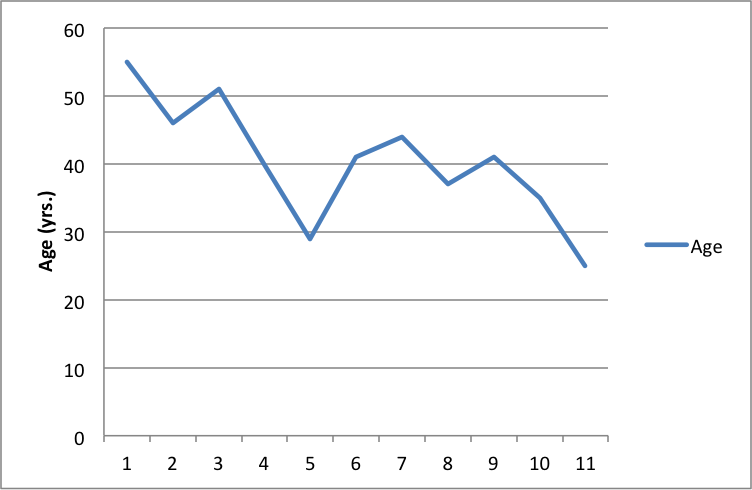
\includegraphics[width=10cm]{figure/example.png} % width can be adjusted
        }
        \caption[คำบรรยายนี้จะโชว์ที่สารบัญ] % This caption will be shown at table of content
        {คำบรรยายนี้โชว์ใต้รูป จาก \href{https://www.google.com} {https://www.google.com}} 
        \label{fig:x1} % label for referencing , ID need to be unique!!
        % fig:.. for figures and tbl:.. for table
    \end{figure}

    \begin{figure}[!h] 
        \centering
        \fbox{
            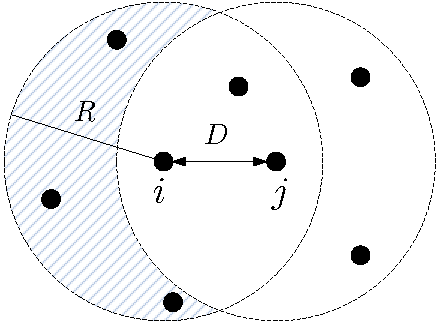
\includegraphics[width=6cm]{figure/example.pdf} % pdf file can also be used as figure
        }
        \caption[คำบรรยายนี้จะโชว์ที่สารบัญ (2)] %
        {คำบรรยายนี้โชว์ใต้รูป} 
        \label{fig:x2} 
    \end{figure}

\pagebreak %% use pagebreak to make content start at new page
% \newpage %% \newpage can also be used

\section{วัตถุประสงค์}
    \emph{
        \begin{flushleft}
            ระบุสิ่งท่ี่จะทำในโครงการ ซึ่งจะใช้สำหรับการประเมินว่าโครงงานทำสำเร็จหรือไม่
        \end{flushleft}
        \begin{flushleft}
            Explain the motivations of your works.    
        \end{flushleft}
        %% How-to: Add bullet points
        %% - use \begin{itemize}... \end{itemize}
        %% - use \item for each bullet point
        \begin{itemize}
            \item  What are the problems you are addressing? 
            \item  Why they are important?
                \begin{itemize} %% new list can be nested within exisiting list like this
                    \item Explain the essentials
                \end{itemize}
            \item  What are the limitations of existing approaches? 
        \end{itemize}
        You may combine this section with the background section.   
    }

\section{ขอบเขตของโครงงาน}

    %% How-to: Add numbered list
    %% - use \begin{enumerate}... \end{enumerate}
    %% - use \item for each bullet point
    Explain the scope of your works. 
    \emph{
        \begin{itemize}
            \item  What are the problems you are addressing? 
            \item  Why they are important?
            \item  What are the limitations of existing approaches? 
        \end{itemize}
    }

\section{ประโยชน์ที่คาดว่าจะได้่รับ}
    \emph{
        โครงงานนี้จะเป็นประโยชน์กับใคร ยังไง ทั้งในเชิงรูปธรรมและนามธรรม ในปัจจุบันหรือในอนาคตถ้านำไปต่อยอด
    }

\pagebreak

\section{ตารางการดำเนินงาน}

    %% Example gantt chart
    \begin{table}[H] % Tips: In contrast to !h, use H to lock placement for the element
        \centering
        \caption{ตารางการดำเนินการในภาคการศึกษาที่ 1}\label{tbl:gantt1}
        \begin{ganttchart}[
                vgrid={*{3}{gray, dotted}, *1{black, dashed}},
                bar label node/.append style={
                align=left,
                text width=width("7. จัดทำรายงานของภาคการศึกษาที่ 1")}
           ]{1}{20}
            \gantttitle{สิงหาคม}{4} \gantttitle{กันยายน}{4} \gantttitle{ตุลาคม}{4} \gantttitle{พฤศจิกายน}{4} \gantttitle{ธันวาคม}{4} \\
            \ganttbar{1. ศึกษาค้นคว้า วิเคราะห์หาปัญหาและที่มา}{2}{2} \\
            \ganttbar{2. เสนอหัวข้อโครงงาน}{3}{3} \\
            \ganttbar{3. ศึกษาค้นคว้า หาข้อมูลที่เกี่ยวข้อง}{3}{4} \\
            \ganttbar{4. นำเสนอโครงการให้กับอาจารย์ที่ปรึกษา}{4}{4} \\
            \ganttbar{5. จัดทำข้อเสนอโครงการ}{5}{9} \\
            \ganttbar{6. นำเสนอข้อเสนอโครงการ}{11}{11} \\
            \ganttbar{7. จัดทำรายงานของภาคการศึกษาที่ 1}{5}{16} \\
            \ganttbar{8. วิเคราะห์และออกแบบ UX/UI}{6}{16} \\
            \ganttbar{9. พัฒนาซอฟต์แวร์และระบบ}{11}{20} \\
            \ganttbar{10. ทดสอบการทำงานของระบบ จากการใช้งานจริงครั้งที่ 1}{17}{20} \\
            \ganttbar{11. นำเสนอและรายงานโครงการของภาคการศึกษาที่ 1}{17}{18} \\
        \end{ganttchart}
    \end{table}


%%%%%%%%%%%%%%%%%%%%%%%%%%%%%%%%%%%%%%%%%%%%%%%%%%%%%%%%%%%%
%%%%%%%%%%%%%%  Literature Review %%%%%%%%%%%%%%%%%%%%%%%%%%
%%%%%%%%%%%%%%%%%%%%%%%%%%%%%%%%%%%%%%%%%%%%%%%%%%%%%%%%%%%%
\chapter{ทฤษฎีความรู้และงานที่เกี่ยวข้อง}

\emph{หัวข้อต่าง ๆ ในแต่ละบทเป็นเพียงตัวอย่างเท่านั้น หัวข้อที่จะใส่ในแต่ละบทขึ้นอยู่กับโปรเจคของนักศึกษาและอาจารย์ที่ปรึกษา}

ในบทที่ 2 จะกล่าวถึง ทฤษฎีที่เกี่ยวข้องที่ใช้ในการทำงานและการศึกษาเพื่อบรรลุวัตถุประสงค์ การอธิบายคำศัพท์หรือภาษาทางคอมพิวเตอร์ที่ได้กล่าวถึงและใช้งานในการแก้ไขปัญหา รวมไปถึงงานวิจัยหรือโครงงานที่ได้ใช้อ้างอิงในการทำงาน

\section{ทฤษฎีที่เกี่ยวข้อง}
    \subsection{Separation of Concern}

        %% How-to: Cite reference
        %% - use \cite{} along with key you assign in .bib file
        \begin{flushleft}
        หลักการ Separation of Concern (SoC Principle) เป็นแนวคิดพื้นฐานในด้านวิศวกรรมซอฟต์แวร์และการออกแบบ โดยเน้นถึงความจำเป็นในการแบ่งระบบที่ซับซ้อนออกเป็นส่วนที่แตกต่างกันและจัดการได้ ซึ่งแต่ละส่วนจะกล่าวถึงลักษณะเฉพาะของฟังก์ชันการทำงาน (function) หรือภาระหน้าที่ (concern หรือ responsibility)~\cite{nattawat20}
        \end{flushleft}
        \begin{flushleft}
        หลักการนี้มีบทบาทสำคัญในการปรับปรุงคุณภาพซอฟต์แวร์ การบำรุงรักษา และความสามารถในการขยาย~\cite{dijkstra82} ในขอบเขตของสถาปัตยกรรมซอฟต์แวร์ การแยกข้อกังวลมักจะเกี่ยวข้องกับการแบ่งระบบออกเป็นโมดูล (modules) หรือส่วนประกอบ (components) โดยแต่ละส่วนจะเกี่ยวข้องกับลักษณะเฉพาะของแอปพลิเคชันเช่น ส่วนติดต่อผู้ใช้ การจัดเก็บข้อมูล หรือตรรกะทางธุรกิจ
        \end{flushleft}
        แนวทางนี้จะลดการพึ่งพาซึ่งกันและกันระหว่างส่วนต่างๆ ของซอฟต์แวร์ ทำให้ง่ายต่อการพัฒนา แก้ไข และดีบักซอฟต์แวร์ เนื่องจากการเปลี่ยนแปลงในด้านหนึ่งมีโอกาสน้อยที่จะส่งผลกระทบต่อส่วนอื่น ๆ มันส่งเสริมฐานรหัสที่มีการจัดระเบียบและเข้าใจได้มากขึ้น ซึ่งอำนวยความสะดวกในการทำงานร่วมกันระหว่างนักพัฒนา
        \begin{flushleft}
        ตามความเห็นในของ \textit{Meyer}~\cite{meyer88} การสร้างซอฟต์แวร์ที่เป็นคุณภาพและมั่นคงคือการรักษาความเข้าใจและความถูกต้องของประสิทธิภาพของแต่ละส่วนในระบบ หนึ่งการพัฒนาที่มีแนวคิดในเรื่องนี้คือการใช้หลักการการแยกปัญหาที่ชัดเจนในองค์กร การเป็นที่รู้ในประเด็นนี้และปรับใช้หลักการการแยกปัญหาอย่างมีประสิทธิภาพสามารถนำไปสู่การพัฒนาระบบซอฟต์แวร์ที่มีประสิทธิภาพและเครื่องมือที่มีคุณภาพสูง
        \end{flushleft}

\section{โครงงานหรืองานวิจัยที่เกี่ยวข้อง}
    \subsection{IPST Program Grader}
    \begin{flushleft}
    \href{https://programming.in.th}{IPST Program Grader} เป็นเว็บไซต์ แอปพลิเคชันที่สร้างขึ้นโดย\textit{สถาบันส่งเสริมการสอนวิทยาศาสตร์และเทคโนโลยี (หรือ สสวท.)}~\cite{ipstGrader} ถูกนำมาปรับปรุงใหม่โดยกลุ่มนักเรียนค่ายโอลิมปิกวิชาการคอมพิวเตอร์ในช่วงปีหลัง ๆ สร้างขึ้นมาเพื่อให้ผู้ใช้สามารถเข้ามาฝึกฝนทักษะการเขียนโปรแกรม เรียนรู้การเขียนโปรแกรม เรียนรู้เกี่ยวกับโครงสร้างข้อมูล และฝึกเขียนอัลกอริทึมที่มีประสิทธิภาพ
    \end{flushleft}
    \begin{flushleft}
    เว็บไซต์นี้มีฐานข้อมูลโจทย์ปัญหาที่แต่งโดยทางสสวท. ที่ผู้ใช้สามารถกดเลือกเข้าไปทำข้อไหนก็ได้ มีระบบสมัครสมาชิก และมี learning resource สำหรับให้ผู้ใช้ได้อ่าน ได้ฝึกฝน ทำความเข้าใจและเรียนรู้การเขียนโปรแกรม 
    \end{flushleft}
    \begin{itemize}
        \item \textbf{ข้อดี}
        \begin{enumerate}
            \item เว็บไซต์มีระบบการตรวจและประเมินผลโปรแกรมที่รวดเร็ว ผู้ใช้สามารถรับรู้ผลได้ทันที
            \item ส่วนประสานผู้ใช้ (User Interface) ถูกออกแบบมาอย่างดี เพื่อความสะดวกสบายของผู้ใช้
            \item เว็บไซต์มีโจทย์ปัญหาที่หลากหลาย แต่งแต่ระดับง่ายสุด ไปยังระดับการแข่งขันระดับนานาชาติ
            \item เว็บไซต์มีระบบจัดหมวดหมู่โจทย์ปัญหา ทำให้ผู้ใช้หาโจทย์ปัญหาที่ต้องการทำได้ง่าย
        \end{enumerate}
        \pagebreak
        \item \textbf{ข้อเสีย}
        \begin{enumerate}
            \item เว็บไซต์ไม่สามารถจะใช้งานเครือข่ายเฉพาะได้ เพราะเว็บไซต์ดังกล่าวอยู่ในเครือข่ายสาธารณะ ทำให้เว็บไซต์นี้ไม่สามารถนำมาใช้ในการแข่งขันภายในได้
            \item ไม่มีระบบสื่อสาร ไม่มีระบบกระทู้สนทนา ไม่มีช่องทางการสื่อสารให้ผู้ใช้ได้คุยปรึกษากันเรื่องโจทย์
            \item ผู้ใช้ไม่สามารถเพิ่มโจทย์ปัญหาเองได้ โจทย์ปัญหาถูกควบคุมและเพิ่มโดยผู้ดูแลเว็บเท่านั้น
        \end{enumerate}
    \end{itemize}
    
\pagebreak
\section{ภาษาคอมพิวเตอร์เเละเทคโนโลยี}
    \subsection{ภาษาคอมพิวเตอร์}
    
    \subsection{เครื่องมือ}
        \subsubsection{React}
            \begin{flushleft}
                React เป็นไลบรารี JavaScript ที่ถูกพัฒนาขึ้นโดย Facebook สำหรับสร้าง User Interface (UI) ที่ได้รับความนิยมอย่างแพร่หลายในการพัฒนาเว็บแอปพลิเคชัน (web applications)~\cite{flanagan20js}
            \end{flushleft}
            \begin{figure}[H]
                \centering
                % \fbox{
                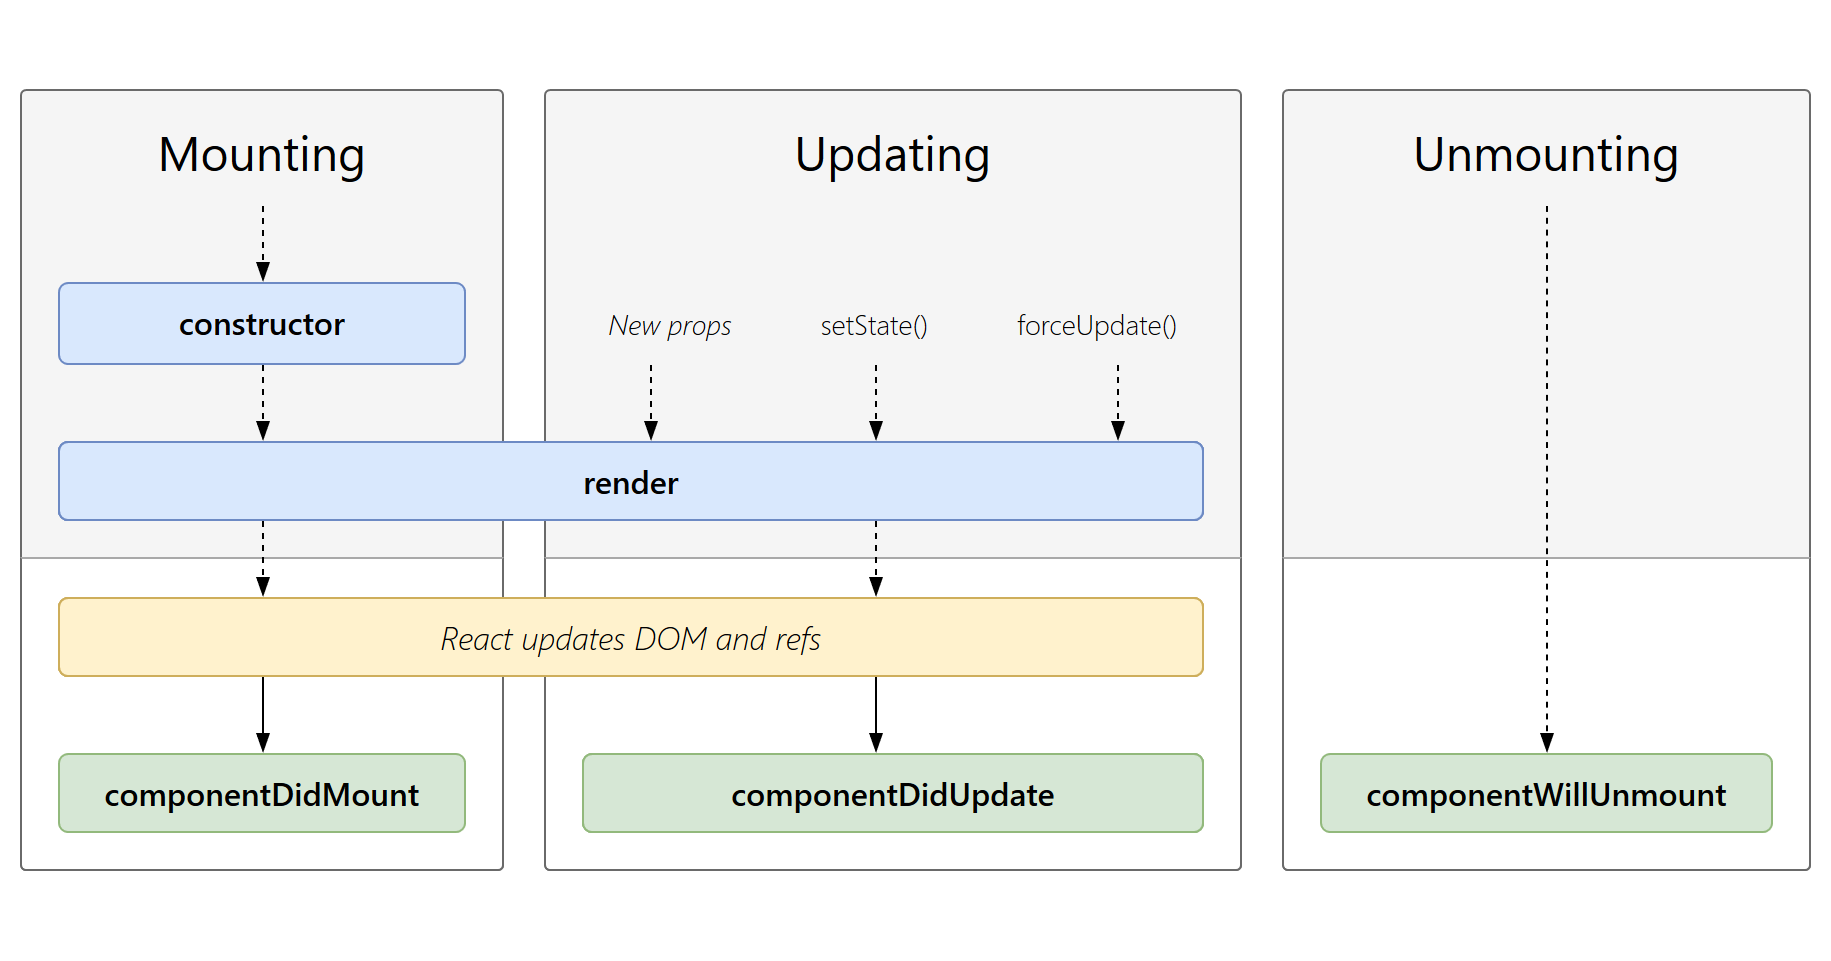
\includegraphics[width=12cm]{figure/literature/react-lifecycle.png}
                % }
                \caption[วัฏจักรการทำงานของ React]{วัฎจักรการ Render, Mount-Unmount และ Update ของ React (React Lifecycle) จาก \href{https://projects.wojtekmaj.pl/react-lifecycle-methods-diagram/}{projects.wojtekmaj.pl} }\label{fig:lit-react}
            \end{figure}
            \begin{flushleft}
                React ให้เครื่องมือและโครงสร้างที่สำหรับการสร้าง UI components ที่หลากหลายและมีประสิทธิภาพ~\cite{crockford08js} หนึ่งในข้อได้เปรียบของ React อยู่ที่การใช้ Virtual DOM ที่ช่วยเพิ่มประสิทธิภาพของการ render องค์ประกอบของ UI และการสร้างแอปพลิเคชันที่มีประสิทธิภาพและสามารถบริหารจัดการ state ของแอปพลิเคชันได้ง่าย~\cite{flanagan20js}
            \end{flushleft}

    \subsection{เทคโนโลยี}
        \subsection{เครื่องคณิตกรณ์ ระบบปฎิบัติการวินโดว์ 11}
        \subsection{แป้นพิมพ์ดีดตัวอักขระเชิงเครื่องกล}

%%%%%%%%%%%%%%%%%%%%%%%%%%%%%%%%%%%%%%%%%%%%%%%%%%%%%
%%%%%%%%%%%%% Design and Methodologies %%%%%%%%%%%%%%
%%%%%%%%%%%%%%%%%%%%%%%%%%%%%%%%%%%%%%%%%%%%%%%%%%%%%
\chapter{วิธีการดำเนินงาน}

\emph{หัวข้อต่าง ๆ ในแต่ละบทเป็นเพียงตัวอย่างเท่านั้น หัวข้อที่จะใส่ในแต่ละบทขึ้นอยู่กับโปรเจคของนักศึกษาและอาจารย์ที่ปรึกษา}


ตัวอย่างการใส่อ้างอิงที่มา -> \cite{hypersense} ถ้าต้องการใส่แหล่งอ้างอิงมากกว่า 1 ให้ทำดังนี้ -> \cite{hypersense,bworld} 
Explain the design (how you plan to implement your work) of your project. Adjust the section titles below to suit the types of your work. Detailed physical design like circuits and source codes should be placed in the appendix.

\section{ข้อกำหนดและความต้องการของระบบ}

\section{สถาปัตยกรรมระบบ}

    %% Example Table 1: For more details see https://www.overleaf.com/learn/latex/Tables
    \begin{table}[!h]
        \centering
            \caption{test table x1}\label{tbl:symbols}
            \begin{tabular}{@{}p{0.07\textwidth}|p{0.7\textwidth}p{0.1\textwidth}}\hline
                \multicolumn{2}{l}{\textbf{SYMBOL}}  & \textbf{UNIT} \\ \hline 
                $\alpha$ & Test variable\hfill & m$^2$ \\
                $\lambda$ & Interarrival rate\hfill &  jobs/second\\
                $\mu$ & Service rate\hfill & jobs/second \\ \hline
            \end{tabular}
        %\begin{tabular}{c|c} \hline
        % $\alpha$ & $\beta$ \\ \hline
        % $\delta$ & $\mu$ \\ \hline
        %\end{tabular}
    \end{table}


\section{Hardware Module 1}
    \subsection{Component 1}
        \subsubsection{Logical Circuit Diagram} % Tips: use \subsection and \subsubsection to organize your headings

\section{Path Finding Algorithm}

\section{Database Design}
    \subsection{แผนภาพโครงสร้างฐานข้อมูล}

    \subsection{คำอธิบายโครงสร้างฐานข้อมูล}
        \begin{flushleft}
            ในระบบฐานข้อมูลนี้ ประกอบด้วยตารางดังต่อไปนี้
        \end{flushleft}
        \begin{enumerate}
            \item \textbf{User}
                เป็นตารางที่เก็บข้อมูลของผู้ใช้แต่ละคน เช่นอีเมลล์, ชื่อ-นามสกุลขของผู้ใช้ เป็นต้น จากความสัมพันธ์ของตารางดังกล่าว กับตารางอื่น ๆ สามารถสรุปความสัมพันธ์ได้ดังนี้
                \begin{itemize}
        %% How-to: Reference element
        %% - use \ref to refer to element within the report (number get update automatically~ very neat!)
                    % use id (fig:db-user-session) of the element you want to link to
                    \item จากรูปที่~\ref{fig:db-user-session} ผู้ใช้สามารถที่จะเข้าสู่ระบบได้หลายเครื่องพร้อม ๆ กัน ก็คือผู้ใช้เข้าสู่ระบบได้ (has) หลาย Session พร้อมกัน
                    % Example Graph Drawing
                        \begin{figure}[H]
                            \centering 
                            \begin{tikzpicture}[auto,node distance=1.5cm]
                                % First Entity
                                \node[entity] (node1) {User};
                                % Entity's children
                                % [grow=up,sibling distance=3cm]
                                % child {node[attribute] {Attribute 1}}
                                % child {node[attribute] {Attribute 2}}
                                % child[grow=left,level distance=3cm] {node[attribute] {Attribute 3}};
                                
                                % Relationship
                                \node[relationship] (rel1) [right = of node1] {has};
                                % Second Entity
                                \node[entity] (node2) [right = of rel1]	{Session};
                                % Draw an edge between rel1 and node1; rel1 and node2
                                \path (rel1) edge node {\(1\)-\(1\)} 
                                (node1) edge node {\(1\)-\(m\)}	(node2);
                            \end{tikzpicture}
                            \caption[แผนผังแสดงความสัมพันธ์ระหว่างตาราง User และ Session]{แผนผังแสดงความสัมพันธ์ระหว่างตาราง User และ Session}
                            \label{fig:db-user-session} % linking to this element using this id
                        \end{figure}
                \end{itemize}
        \end{enumerate}
                        
    % Example Table 2
    \subsection{พจนานุกรมข้อมูล}
        \begin{table}[!h]
            \centering
            \caption{พจนานุกรมข้อมูลของตาราง User}\label{tbl:data-dict-user}
            \begin{tabular}{p{2cm}|p{4cm}p{2cm}p{3cm}p{2cm}} \hline\hline
                Attribute Name & Description & Data Type & Constraints & References \\ \hline\hline
                id & รหัส ID การส่งงาน & bigint & Primary Key & - \\
                assignment\_id & ID ของภาระงานหรือโจทย์ & bigint & Foreign Key, Not Null & Assignment \\
                user\_id & ID ของผู้ใช้ & varchar(64) & Foreign Key, Not Null & User \\
                language & ภาษาที่ใช้ในการเขียนโค้ด & varchar(64) & Not Null & - \\
                file\_url & ลิงก์ไฟล์งาน & varchar(128) & Not Null & - \\
                submitted\_at & วันเวลาส่งงาน & datetime & Current Timestamp & - \\
                compilation\_log & ผลการคอมไพล์ & longtext & - & - \\ \hline\hline
        \end{tabular}   
    \end{table}

\section{UML Design}

\section{GUI Design}
    

\section{การออกแบบการทดลอง}
    \subsection{ตัวชี้วัดและปัจจัยที่ศึกษา}
    \subsection{รูปแบบการเก็บข้อมูล}

%%%%%%%%%%%%%%%%%%%%%%%%%%%%%%%%%%%%%%%%%%%%%%%%%%%%%%%%%%%%%%
%%%%%%%%%%%%%%%%%%%% Experiments %%%%%%%%%%%%%%%%%%%%%%%%%%%%%
%%%%%%%%%%%%%%%%%%%%%%%%%%%%%%%%%%%%%%%%%%%%%%%%%%%%%%%%%%%%%%%
\chapter{ผลการดำเนินงาน}


\emph{หัวข้อต่าง ๆ ในแต่ละบทเป็นเพียงตัวอย่างเท่านั้น หัวข้อที่จะใส่ในแต่ละบทขึ้นอยู่กับโปรเจคของนักศึกษาและอาจารย์ที่ปรึกษา}

\emph{
    You can title this chapter as \textbf{Preliminary Results} ผลการดำเนินงานเบื้องต้น or \textbf{Work Progress} ความก้าวหน้าโครงงาน for the progress reports. Present implementation or experimental results here and discuss them.
    ใส่เฉพาะหัวข้อที่เกี่ยวข้องกับงานที่ทำ 
}

\section{ประสิทฺธิภาพการทำงานของระบบ} 
\section{ความพึงพอใจการใช้งาน}
\section{การวิเคราะห์ข้อมูลและผลการทดลอง}

%%%%%%%%%%%%%%%%%%%%%%%%%%%%%%%%%%%%%%%%%%%%%%%%%%%%%%%%%%%%%%%
%%%%%%%%%%%%%%%%%%%% Conclusions %%%%%%%%%%%%%%%%%%%%%%%%%%%%%
%%%%%%%%%%%%%%%%%%%%%%%%%%%%%%%%%%%%%%%%%%%%%%%%%%%%%%%%%%%%%%%
\chapter{บทสรุป}


\emph{หัวข้อต่าง ๆ ในแต่ละบทเป็นเพียงตัวอย่างเท่านั้น หัวข้อที่จะใส่ในแต่ละบทขึ้นอยู่กับโปรเจคของนักศึกษาและอาจารย์ที่ปรึกษา}

This chapter is optional for proposal and progress reports but 
is required for the final report.

\section{สรุปผลโครงงาน}
    \emph{
        สรุปว่าโครงงานบรรลุตามวัตถุประสงค์ที่ตั้งไว้หรือไม่ อย่างไร   
    }

\section{ปัญหาที่พบและการแก้ไข}
    \emph{
        State your problems and how you fixed them.
    }

\section{ข้อจำกัดและข้อเสนอแนะ}
    \emph{
        ข้อจำกัดของโครงงาน What could be done in the future to make your projects better.
    }

%%%%%%%%%%%%%%%%%%%%%%%%%%%%%%%%%%%%%%%%%%%%%%%%%%%%%%%%%%%%%%%
%%%%%%%%%%%%%%%%%%%% Bibliography %%%%%%%%%%%%%%%%%%%%%%%%%%%%%
%%%%%%%%%%%%%%%%%%%%%%%%%%%%%%%%%%%%%%%%%%%%%%%%%%%%%%%%%%%%%%%

%%%% Comment this in your report to show only references you have
%%%% cited. Otherwise, all the references below will be shown.
%\nocite{*}
%% Use the kmutt.bst for bibtex bibliography style 
%% You must have cpe.bib and string.bib in your current directory.
%% You may go to file .bbl to manually edit the bib items.

% Sept, 2021 by Thanin
% improve url breaks to prevent unnecessary big white spaces in some cases
\makeatletter
\g@addto@macro{\UrlBreaks}{\UrlOrds}
\makeatother
% 

\bibliographystyle{kmutt} %% Bibliography style: need to be pointing to kmutt.bst
\bibliography{main} %% Name of .bib file you're using, can be change :)

%%%%%%%%%%%%%%%%%%%%%%%%%%%%%%%%%%%%%%%%%%%%%%%%%%%%%%%%%%%%%%%
%%%%%%%%%%%%%%%%%%%%%%%% Appendix %%%%%%%%%%%%%%%%%%%%%%%%%%%%%
%%%%%%%%%%%%%%%%%%%%%%%%%%%%%%%%%%%%%%%%%%%%%%%%%%%%%%%%%%%%%%%
\appendix{ชื่อภาคผนวกที่ 1}
\noindent{\large\bf ใส่หัวข้อตามความเหมาะสม} \\

    This is where you put hardware circuit diagrams, detailed experimental data in tables or source codes, etc.. \\ \bigskip

    \begin{figure}[!h]
        \caption{This is the figure x11 ทดสอบ จาก \href{https://www.google.com} {https://www.google.com}}\label{fig:x1}
    \end{figure}

%% Example Appendix 1: Writing math equation
This appendix describes two static allocation methods for fGn (or fBm)
traffic. Here, $\lambda$ and $C$ are respectively the traffic arrival
rate and the service rate per dimensionless time step. Their unit are
converted to a physical time unit by multiplying the step size
$\Delta$. For a fBm self-similar traffic source,
Norros~\cite{norros95} provides its EB as
\begin{equation}\label{eq:norros}
  C = \lambda + (\kappa(H)\sqrt{-2\ln\epsilon})^{1/H}a^{1/(2H)}x^{-(1-H)/H}\lambda^{1/(2H)}
\end{equation}
where $\kappa(H) = H^H(1-H)^{(1-H)}$. Simplicity in the calculation is
the attractive feature of (\ref{eq:norros}).

The MVA technique developed in~\cite{kim01} so far provides the most
accurate estimation of the loss probability compared to previous
bandwidth allocation techniques according to simulation results.
Consider a discrete-time queueing system with constant service rate
$C$ and input process $\lambda_n$ with $\mathbb{E}\{\lambda_n\} =
\lambda$ and $\mathrm{Var}\{\lambda_n\} = \sigma^2$.  Define $X_n \equiv
\sum_{k=1}^n \lambda_k - Cn$.  The loss probability due to the MVA
approach is given by
\begin{equation}\label{eq:loss_mva}
  \varepsilon \approx \alpha e^{-m_x/2}
\end{equation}
where
\begin{equation}\label{eq:mx}
m_x = \min_{n \geq 0} \frac{((C-\lambda)n + B)^2}{\mathrm{Var}\{X_n\}} =
\frac{((C-\lambda)n^\ast + B)^2}{\mathrm{Var}\{X_{n^{\ast}}\}}
\end{equation} 
and 
\begin{equation}\label{eq:alpha}
  \alpha =
  \frac{1}{\lambda\sqrt{2\pi\sigma^2}}\exp\left(\frac{(C-\lambda)^2}{2\sigma^2}\right)
  \int_C^\infty (r-C)\exp\left(\frac{(r-\lambda)^2}{2\sigma^2}\right)\, dr
\end{equation}
For a given $\varepsilon$, we numerically solve for $C$ that satisfies
(\ref{eq:loss_mva}). Any search algorithm can be used to do the task.
Here, the bisection method is used.  

Next, we show how $\mathrm{Var}\{X_n\}$ can be determined.  Let
$C_{\lambda}(l)$ be the autocovariance function of $\lambda_n$.  The
MVA technique basically approximates the input process $\lambda_n$
with a Gaussian process, which allows $\mathrm{Var}\{X_n\}$ to be
represented by the autocovariance function.  In particular, the
variance of $X_n$ can be expressed in terms of $C_{\lambda}(l)$ as
\begin{equation}
  \mathrm{Var}\{X_n\} = nC_{\lambda}(0) + 2\sum_{l=1}^{n-1} (n-l)C_{\lambda}(l)
\end{equation} 
Therefore, $C_{\lambda}(l)$ must be known in the MVA technique, either
by assuming specific traffic models or by off-line analysis in case of
traces.  In most practical situations, $C_{\lambda}(l)$ will not be
known in advance, and an on-line measurement algorithm developed
in~\cite{eun01} is required to jointly determine both $n^\ast$ and
$m_x$. For fGn traffic, $\mathrm{Var}\{X_n\}$ is equal to $\sigma^2
n^{2H}$, where $\sigma^2 = \mathrm{Var}\{\lambda_n\}$, and we can find
the $n^\ast$ that minimizes (\ref{eq:mx}) directly. Although $\lambda$
can be easily measured, it is not the case for $\sigma^2$ and $H$.
Consequently, the MVA technique suffers from the need of prior
knowledge traffic parameters.


%%%%%%%%%%%%%%%%%%%%%%%%%%%%%%%%%%%%%%%%%%%%%%%%%%%%%%%%%%
%%%%%%%%%%%%%%% The 2nd appendix %%%%%%%%%%%%%%%%%%%%%%%%%%
%%%%%%%%%%%%%%%%%%%%%%%%%%%%%%%%%%%%%%%%%%%%%%%%%%%%%%%%%%
\appendix{ชื่อภาคผนวกที่ 2}
\noindent{\large\bf ใส่หัวข้อตามความเหมาะสม} \\

%% Example Appendix 2
    Next, we show how $\mathrm{Var}\{X_n\}$ can be determined.  Let
    $C_{\lambda}(l)$ be the autocovariance function of $\lambda_n$.  The
    MVA technique basically approximates the input process $\lambda_n$
    with a Gaussian process, which allows $\mathrm{Var}\{X_n\}$ to be
    represented by the autocovariance function.  In particular, the
    variance of $X_n$ can be expressed in terms of $C_{\lambda}(l)$ as
    \begin{equation}
      \mathrm{Var}\{X_n\} = nC_{\lambda}(0) + 2\sum_{l=1}^{n-1} (n-l)C_{\lambda}(l)
    \end{equation} 
    
    \noindent{\large\bf Add more topic as you need} \\
    
    Therefore, $C_{\lambda}(l)$ must be known in the MVA technique, either
    by assuming specific traffic models or by off-line analysis in case of
    traces.  In most practical situations, $C_{\lambda}(l)$ will not be
    known in advance, and an on-line measurement algorithm developed
    in~\cite{eun01} is required to jointly determine both $n^\ast$ and
    $m_x$. For fGn traffic, $\mathrm{Var}\{X_n\}$ is equal to $\sigma^2
    n^{2H}$, where $\sigma^2 = \mathrm{Var}\{\lambda_n\}$, and we can find
    the $n^\ast$ that minimizes (\ref{eq:mx}) directly. Although $\lambda$
    can be easily measured, it is not the case for $\sigma^2$ and $H$.
    Consequently, the MVA technique suffers from the need of prior
    knowledge traffic parameters. 

\end{document}
